% !TEX TS-program = xeLaTeX
\documentclass[aspectratio=169]{beamer}

% Package imports
\usepackage{fontspec}
\usepackage{epigraph}
\usepackage{xcolor}
\usepackage[percent]{overpic}

% custom options to make epigraph look good on a beamer slide
\renewcommand{\epigraphrule}{0pt}
\setlength{\epigraphwidth}{.9\textwidth}
\renewcommand{\textflush}{flushepinormal}

\newcommand\blfootnote[1]{%
  \begingroup
  \renewcommand\thefootnote{}\footnote{#1}%
  \addtocounter{footnote}{-1}%
  \endgroup
}

% default document font specifications
\setmainfont{FiraSans-Book}
\setsansfont{FiraSans-Book}
\definecolor{textcolour}{rgb}{255,255,255}

% Definign the Mozilla colour palette for presentations 
\definecolor{moz_dark_green}{RGB}{77,78,83}
\definecolor{moz_light_green}{RGB}{208,211,212}
\definecolor{moz_light_blue}{RGB}{0,150,221}
\definecolor{moz_dark_blue}{RGB}{0,33,71}
\definecolor{moz_accent_green}{RGB}{111,190,74}
\definecolor{moz_accent_yellow}{RGB}{255,203,0}
\definecolor{moz_accent_orange}{RGB}{255,149,0}
\definecolor{moz_accent_orange2}{RGB}{230,96,0}
\definecolor{moz_accent_red}{RGB}{193,56,50}

% new counter for column enumerates
\newcounter{savedenum}
\newcommand*{\saveenum}{\setcounter{savedenum}{\theenumi}}
\newcommand*{\resume}{\setcounter{enumi}{\thesavedenum}}

% Background for all slides set here
\setbeamertemplate{background canvas}{
\includegraphics [width=\paperwidth]{bg_alt_small.png}}

\setbeamercolor{structure}{fg=textcolour}

\setbeamerfont{title}{size = \Huge}
\setbeamercolor{normal text}{fg=textcolour}

%define specific fint size interpretations for the beamer presentation mode.
\renewcommand{\tiny}{\fontsize{7pt}{8pt}\selectfont}
\renewcommand{\scriptsize}{\fontsize{9pt}{12pt}\selectfont}
\renewcommand{\footnotesize}{\fontsize{10pt}{12pt}\selectfont}
\renewcommand{\small}{\fontsize{12pt}{18pt}\selectfont}
\renewcommand{\normalsize}{\fontsize{14pt}{18pt}\selectfont}
\renewcommand{\large}{\fontsize{16pt}{24pt}\selectfont}
\renewcommand{\Large}{\fontsize{24pt}{37pt}\selectfont}
\renewcommand{\LARGE}{\fontsize{36pt}{48pt}\selectfont}
\renewcommand{\huge}{\fontsize{48pt}{54pt}\selectfont}
\renewcommand{\Huge}{\fontsize{80pt}{96pt}\selectfont}

% remove navigation symbols
\setbeamertemplate{navigation symbols}{}
    
\begin{document}


\begin{frame}
\frametitle{The Morphology of the Web is Changing!}

% hey Data natives! it is absolutely great to be back for another iteration of this conference. 
%My name is Martin Lopatka, I work on Research Engineering and Data Science at Mozilla! 
%I'm here to talk to you about the Biggest data I know of...  The world’s largest shared public resource... The Web.
% So, we at Mozilla, work a bit on the web, we build a web browser, you may have heard of it.. it's called Firefox. 
% And, so as part of that, I'd say a pretty important part of that is knowing a thing or two about the World Wide Web.
% the story i want to talk about today has to do with its shape and a little bit about the technologies that define that shape
% One definition of Morphology is "the study of form and structure without consideration of function"

\begin{overpic}[width=0.7\textwidth]{morphs.png}
\put(45, 0){Form and structure of the modern Web} 
\end{overpic}

% So what got me started down this road: well a couple fo years ago, maybe around...  July 6th, 2016... at 11:16am.. Our VP of product Nick Nguyen made a medium post about the state of the web, 
\end{frame}

\begin{frame}
\frametitle{Disclaimer}
Martin Lopatka provides this contribution to the Data Natives 2018 conference in a personal capacity. The views expressed are his own and do not necessarily represent the views of Mozilla Corporation or the Mozilla Foundation.

% In addition on a personal note, this talk is not meant to be a vilification of the advertisement industry, or big companies, social media platforms, content publishers, or any other party. But rather, I want to focus on the changing nature fo the Web and what it means for technology and for people.
\end{frame}

{
\usebackgroundtemplate{
\includegraphics[width=\paperwidth]{bg_alt_small-rlogo.png}}%
\begin{frame}
\begin{overpic}[width=0.7\textwidth]{2003-web-small.png}
\put(-05,90){\textbf{THE INTERNET 2003}}
\put(-05,86){\tiny{Barrett Lyon / The Opte Project}}
\end{overpic}
% Op-tee project visualization made by a massive crawl fo the web, The colors were based on Class A allocation of IP space to different registrars in the world.
% This map from opte was generated based on a 2003 crawl of the web a time where there were approximately 30, million TLDs registered.
% reported by the Internet Systems Consortium.

% at this time, a large portion of the links on a page were placed there by the content creators. The individuals that 
\end{frame}
}

{
\usebackgroundtemplate{
\includegraphics[width=\paperwidth]{bg_alt_small-rlogo.png}}%
\begin{frame}
\begin{overpic}[width=0.8\textwidth]{2015-web-large-2.png}
\put(-04.5,69.5){\textbf{THE INTERNET 2015}}
\put(-04.5,66){\tiny{Barrett Lyon / The Opte Project}}
%\blfootnote{Barrett Lyon / The Opte Project}
\end{overpic}
% By now the Web includes over 314 Million top level domains registered  
% https://www.verisign.com/ annual domain registrar market briefs
\end{frame}
}

\begin{frame}
\frametitle{The Centrality of Advertisers}
\large{Are trackers the new backbone of the Web?}
\begin{center}
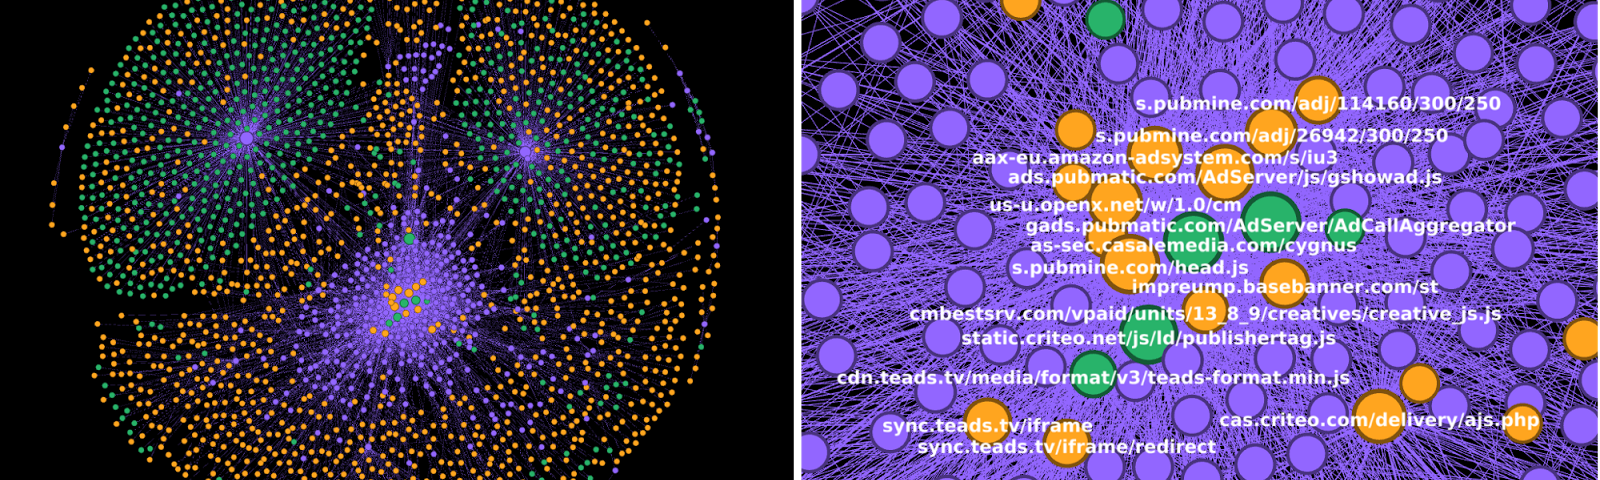
\includegraphics[width=0.85\paperwidth]{0thN-8lZ4H2_xjbkt.png}
\end{center}
% In 2017 we started working with students at the Information and Language Processing systems group at the University of Amsterdam, exploring the role of highly connected, hub nodes, among the most popular (or highly visited) websites on the Web at that time.

% As seen in the 2015 snapshot of the Web, we observed some hyper-connected nodes naturally 

% Community detection was performed using Louvain Modularity, which groups nodes within a network that are more densely connected to one another than to other nodes. This was performed using third-party resources as the network’s edges; not the hyperlinks
% Jelmer Neeven, University of Amsterdam.

% In some examples, we observed substantially fewer hyperlinks between pages belonging to separate tracking communities than between pages tracked by a single % source of third-party resources. As the dynamic link generation is intended to keep attention in-ecosystem. This is the first indication 
\end{frame}

{
\usebackgroundtemplate{
\includegraphics[width=\paperwidth]{bg_alt_small-rlogo.png}}%
\begin{frame}
\frametitle{How did we get to an ecosystem of silos?}
%We’ve already made some scary discoveries about the diversity of browsing behaviour. A very early examination of a small group of Firefox users’, who voluntarily shared their browsing history via an opt-in data science program called Firefox Pioneer (I'm happy to talk more about that after the talk).
\begin{itemize}
\item{40\% of total Web browsing page views can be attributed to only 65 top level domains}
\item{Five (TLD+1) sites (Google, Facebook, Amazon, Yahoo, and Reddit) make up 22\% of all traffic
\footnote{https://medium.com/firefox-context-graph/are-trackers-the-new-backbone-of-the-web-fb800435da15}}
% Based on Pioneers' actual web browsing behaviour during a fixed length data collection period in 2016.
\item{Of the 22,310,889 domains processed, 52.63\% (11,742,112) were found to serve ads
\footnote{https://commecica.com/2018/06/27/web-ad-prevalence/}}
%In a study performed by "Comme ci comme ca" using the May 2018 batch of common crawl formats and comparing links against the Easylist ruleset file (which is the basis of how the line of Adblock adblocker browser extensions work.


% buisness model does not depend as much on 
\end{itemize}
\end{frame}
}

\begin{frame}
\frametitle{}
\epigraph{Social platforms were designed to facilitate; they became attention brokers, they are designed to help companies reach users as these sort of middlemen where they know a ton about you and thats the service they are providing to the advertisers.}{Renee DiResta "The Internet's Original Sin\\ 27-Oct-2018 12:45}
% Ads alone aren't a problem, targeting is the problem. Social platforms are designed to collect attention and information in order to sell them to advertisers
% according to research cited in that talk 60% of people in the US get their news from Facebook. 
% In order to continue to be effective as an *infrastructure for advertisement* content and social platforms have evolved to maximise sustained engagement. That is a critical terms. Notice that no part of an engagement-based optimisation favours quality, but rather popularity.

% We will get back to this idea of "random walk models" 
\end{frame}

\begin{frame}
\frametitle{}
%in 2018, Mulligan and Griffin, published an essay in the GEORGETOWN LAW TECHNOLOGY REVIEW, explaining the disconnect between peoples expectation of Google and other search providers as stewards of knowledge. And compared these operational assumptions with the algorithmic reality of search ending first page results. 
The highest trafficked pages on the Web are search engines, Social media platforms, and Commerce platforms
\begin{columns}[T]
  \begin{column}{.5\linewidth}
  \begin{enumerate}
	\item{Google.com}
	\item{Youtube.com}
	\item{Facebook.com}
	\item{Baidu.com}
	\item{Wikipedia.org $\star$}
    \saveenum
  \end{enumerate}
  \end{column}
  \begin{column}{.5\linewidth}
  \begin{enumerate}
    \resume
         \item{Qq.com}
	\item{Taobao.com}
	\item{Yahoo.com}
	\item{Tmall.com}
	\item{Amazon.com}  
	\end{enumerate}
  \end{column}
\end{columns}
%RESCRIPTING SEARCH TO RESPECT THE RIGHT TO TRUTH
%Deirdre K. Mulligan* and Daniel S. Griffin**

%With the exception of Wikipedia, these sites are all designed to maximise time on page. And 
\end{frame}

\begin{frame}
\frametitle{}
\epigraph{The problem is that the web is no longer built upon the simple premise of a collection of small static HTML and image files served up with a simple tag structure and readily parsed with a few lines of code. Today’s web is richly dynamic, multimedia and increasingly broken into walled gardens and device-specific parallel webs.}{Kalev Leetaru "Are Web Archives Failing The Modern Web: Video, Social Media, Dynamic Pages and The Mobile Web"\\ 24-Feb-2017 22:41}
% 
\end{frame}
\begin{frame}
\frametitle{The new ecology of outbound links}
\begin{itemize}
\item{Retargeting}
\item{advertisement}
\item{realtime bidding}
\item{social linking}
\end{itemize}
\end{frame}

\begin{frame}
\frametitle{}
\epigraph{I can't help but feel nauseous when I am loading independent.co.uk, Firefox literally grinds to a halt because of the extreme amount of tracking requests being logged in the browser console, and a popup shows up and says "We value your privacy"}{motin \\
28-Oct-2018 11:37}
%\blfootnote{https://github.com/motin}
\end{frame}

\begin{frame}
transparency, technology, education

%Popularized by Berners-Lee's book Weaving the Web[32] and a Scientific American article by Berners-Lee, James Hendler, and Ora Lassila,[33] the term Semantic Web describes an evolution of the existing Web in which the network of hyperlinked human-readable web pages is extended by machine-readable metadata about documents and how they are related to each other, enabling automated agents to access the Web more intelligently and perform tasks on behalf of users. This has yet to happen. In 2006, Berners-Lee and colleagues stated that the idea "remains largely unrealized".[34]

% meaning that web crawls in the future will face the difficulty of increasingly complex algorithmic generation of outbound links.
% as the sophistication of 
\end{frame}

\begin{frame}
\frametitle{Challenges to crawl technology}
\begin{itemize}
\item{Limited View - the open web makes up less and less of the Web. Content Silos}
\item{Dynamic content serving}
\item{Walled gardens}
\end{itemize}
% meaning that web crawls in the future will face the difficulty of increasingly complex algorithmic generation of outbound links.
% as the sophistication of 
\end{frame}


{
\usebackgroundtemplate{
\includegraphics[width=\paperwidth]{bg_last.png}}%
\begin{frame}

\end{frame}
}




\end{document}
